\documentclass[letterpaper, 10 pt, conference]{article} 
\usepackage[english]{babel}
\usepackage{amsmath,amssymb,amscd,amsthm} % variety of useful math macros
\usepackage[inner=1.5 cm, outer = 1.5 cm, top=1 cm, bottom = 1.5 cm]{geometry}
\usepackage{subcaption}
%For inserting graphics
\usepackage{graphicx}
\usepackage[dvipsnames]{xcolor}
\usepackage{listings}
\usepackage[utf8]{inputenc}
\usepackage{hyperref}
\usepackage{array, multirow}
%For diagrams
%\usepackage{tikz} 
\usepackage{tikz}
\tikzset{
	treenode/.style = {shape=rectangle, rounded corners,
		draw, align=center,
		top color=white, bottom color=blue!20},
	root/.style     = {treenode, font=\Large, bottom color=red!30},
	env/.style      = {treenode, font=\ttfamily\normalsize},
	dummy/.style    = {circle,draw}
}

\newcommand\N{\ensuremath{\mathcal{N}}}		%N for networks
\renewcommand{\P}{\ensuremath{\mathbb{P}}} %P for probability measures
\renewcommand{\iff}{\ensuremath{\Leftrightarrow}} %Shorter \iff 

%\newtheorem{theorem}{Theorem}
\newtheorem{prop}{Proposition}
\newtheorem{lemma}{Lemma}

\lstset{ 
	basicstyle=\footnotesize,        % the size of the fonts that are used for the code
	breakatwhitespace=false,         % sets if automatic breaks should only happen at whitespace
	breaklines=true,                 % sets automatic line breaking
	showspaces=false,                % show spaces everywhere adding particular underscores; it overrides 
	showstringspaces = false,
	stringstyle=\color{MidnightBlue},     % string literal style
	backgroundcolor=\color{White},   
	escapeinside={/*!}{!*/},
	escapebegin=\color{white}
}

\title{Statistical tests}
\author{G. Palafox}


\begin{document}

\maketitle

\begin{abstract}
Elementary facts of statistical tests are presented. Common statistical tests are performed on real data sets.
\end{abstract}

\section{Introduction}
In this report, basic facts about statistical tests are presented, along with examples of tests performed on real data sets of Mexico City subway system. The data was downloaded directly from INEGI's website \cite{inegi}, and includes kilometers traveled, passengers transported, and energy consumed by Mexico City's subway in 2018 and 2019. A fragment of this data is shown in Table \ref{tab:data}. The work was coded in R version 4.0.0 \cite{R} on a Jupyter \cite{jupyter} notebook\footnote{The notebook with the code containing our analysis, as well as this report, can be found in the Github Repository: \url{https://github.com/palafox794/AppliedProbabilityModels/tree/master/Assignment6}}. 

% latex table generated in R 4.0.0 by xtable 1.8-4 package
% Sun Oct 11 13:18:37 2020
\begin{table}
	\centering
	\caption{Fragment of Mexico City subway data.}
	\begin{tabular}{lrrr}
		\hline
		Period & Km traveled (thousands) & Passengers Transported (millions) & Energy consumed (thousands of KWH) \\ 
		\hline
		2018 &  &  &  \\ 
		January & 3816.46 & 129.10 & 89340.53 \\ 
		February & 3389.20 & 124.69 & 80122.84 \\ 
		March & 3688.76 & 131.28 & 89370.53 \\ 
		April & 3646.12 & 132.84 & 84142.34 \\ 
		May & 3768 & 135.99 & 89340.53 \\ 
		\hline
	\end{tabular}
	\label{tab:data}
\end{table}


\section{Statistical hypothesis testing}
The following is a brief summary of the theory regarding statistical hypothesis testing. It is not original work by the author. All presented here, and further topics, can be found in excellent books such as the one by Ross \cite{Ross_2010}, Casella and Berger \cite{Casella_Berger_2002}, or Navarro's online electronic book \cite{Navarro}.
 A statistical hypothesis is a statement about the nature of data, usually in terms of some statistical parameter \cite{Ross_2010}. To test the hypothesis, it must be decided whether a data sample appears to be consistent with said hypothesis For example, it may be the case where the real mean of some data is unknown, and a sample is tested to see if it is consistent with data having mean $m_0$. The hypothesis to be tested is called {\it null hypothesis}, denoted by $H_0$, and the alternative is called \textit{alternative hypothesis}, denoted by $H_1$ or $H_a$. In the previous example, the test would be written as
\begin{equation}
	H_0 : \mu = m_0, \quad H_1 : \mu \neq m_0,
\end{equation}
where $\mu$ denotes the real mean of the population. The alternative hypothesis can also be written as $\mu > m_0$ or $\mu < m_0$. The null hypothesis can also be written as $\mu - m_0 = 0$, which would change the alternative hypothesis to $\mu - m_0 > 0$, and so on. 
The typical set up consists of specifying a small value $\alpha$ (called \textit{significance level}, commonly set as 0.05) and then requiring the test to have the property that, whenever $H_0$ is true, its probability of being rejected is less than or equal to $\alpha$. Statistical tests often output a $p$-value: this is the smallest significance level at which we would allow for the rejection of the null hypothesis for the given data \cite{Navarro, Ross_2010}. 

\subsection{Practical considerations }
When performing statistical tests, certain questions arise, such as choosing significance levels, or interpreting the output of the test. We intend to address some of these questions here, showing examples of statistical tests performed in R.  

\subsubsection{Interpreting the output of a statistical test}
If the $p$-value is less than the significance level $\alpha$, the null hypothesis is rejected and the alternative hypothesis is accepted. On the contrary, if $p \geq \alpha$, we do not reject $H_0$. Rejecting the null hypothesis should be taken as a strong indicative that it does not appear consistent with the observed data \cite{Ross_2010}, while not rejecting $H_0$ is a weak indicative that $H_0$ is consistent with the data \cite{Ross_2010}.
For example, many tests require an assumption of normality. Shapiro-Wilk normality test is a test whose null hypothesis is: \textit{data comes from a normal distribution}.  In R, it is easy to perform this test on a numeric array \texttt{passng} containing the (millions) of passengers transported by Mexico City subway each month. It is shown in Listing \ref{lst:shapiro}. This gives a $p$-value of 0.24. Taking a significance level $\alpha = 0.05$, the $p$-value is greater than $\alpha$, so we do not reject the hypothesis that data comes from a normal distribution, and accept it instead. The same test was performed on different data samples, whose outputs are shown in Table \ref{tab:shapiro}.
\begin{lstlisting}[language=R, caption={Normality test}, label={lst:shapiro} ]
shapiro.test(passng)
#	Shapiro-Wilk normality test

#data:  passng
#W = 0.94795, p-value = 0.2445
\end{lstlisting}


\begin{table}
	\centering
	\caption{$p$-values from Shapiro-Wilk normality test on different data samples.}
	\begin{tabular}{lr}
		\hline
		Data & $p$-value\\ 
		\hline
		Passengers & 0.245 \\ 
		Passengers in 2018 & 0.346 \\ 
		Passengers in 2019 & 0.927 \\ 
		Kilometers traveled & 0.495 \\ 
		Energy consumption & 0.112 \\ 
		\hline
	\end{tabular}
	\label{tab:shapiro}
\end{table}

On the other hand, suppose it is of interest to see whether the number of passengers and the kilometers traveled had the same variance. Fisher's F test can be performed, as seen in Listing \ref{lst:fisher}, and it outputs a $p$-value smaller than $2.2 \times 10^{-16}$. In this case, the null hypothesis is rejected, and the ratio of the variance is assumed to be distinct to one.

\begin{lstlisting}[language=R, caption={Fisher's F test}, label={lst:fisher} ]
var.test(passng, km)

F test to compare two variances

#data:  passng and km
#F = 0.0015576, num df = 23, denom df = 23, p-value < 2.2e-16
#alternative hypothesis: true ratio of variances is not equal to 1
#95 percent confidence interval:
#0.0006738075 0.0036006134
#sample estimates:
#ratio of variances 
#0.001557601 
\end{lstlisting}

\subsubsection{Meaning of rejecting the null hypothesis}
It should be noted that the goal of a statistical test is not to determine whether $H_0$ is true or not, but to determine whether it being true is consistent with the given data \cite{Ross_2010}. Rejecting the null hypothesis should mean that our observed data is very unlikely if $H_0$ is true \cite{Ross_2010}.
Consider the case of performing a One Sample $t$-Test to see whether the mean of passengers transported is \texttt{mu}$ = 100$.  Carrying this out in R (see Listing \ref{lst:one-sample-t-test}) gives a $p$-value smaller than $2.2 \times 10^{-16}$, which leads to rejecting the null hypothesis of the sample having mean equal to a hundred. This means that, if the true mean was 100, it would be very unlikely to observe data as the observed in \texttt{passng}.
\begin{lstlisting}[language=R, caption={One sample t-test.}, label={lst:one-sample-t-test} ]
 t.test(passng, mu = 100)
 #	One Sample t-test
 
 #data:  passng
 #t = 26.513, df = 23, p-value < 2.2e-16
 #alternative hypothesis: true mean is not equal to 100
 #95 percent confidence interval:
 #130.2191 135.3338
 #sample estimates:
 #mean of x 
 #132.7765 
 \end{lstlisting}
 
 A similar conclusion can be reached with Wilcoxon signed rank test, which unlike one sample $t$-test, does not assume a normal distribution for our data. The results are seen in Listing \ref{lst:wilcoxon-signed-rank}, which show a $p$-value of $1.192 \times 10^{-7} < 0.05$.
  \begin{lstlisting}[language=R, caption={Wilcoxon signed rank test.}, label={lst:wilcoxon-signed-rank} ]
wilcox.test(passng, mu=100, conf.inf=TRUE)

#Wilcoxon signed rank exact test

#data:  passng
#V = 300, p-value = 1.192e-07
#alternative hypothesis: true location is not equal to 100
 \end{lstlisting}

\subsubsection{Parametric and non-parametric tests. Assumptions and examples}
Common parametric tests include Student's $t$-test, Pearson's correlation coefficient, linear regression and ANOVAs. Common assumptions for these tests is that observations are independent, and that the samples come from normal distributed populations with common variance. As seen in Listing \ref{lst:correlation}, a correlation test can be used to see whether there is correlation between kilometers traveled and passengers transported. In this case, the null hypothesis is that true correlation is equal to zero. Given how a $p$-value of $0.003 < 0.05$ was obtained, the null hypothesis can be rejected, concluding there is some correlation between the variables. This can be further supported with the graphic in Figure \ref{fig:correlation}, where kilometers traveled are plotted against passengers transported ($x$ and $y$ axis respectively).
 \begin{lstlisting}[language=R, caption={Correlation test.}, label={lst:correlation} ]
 cor.test(km, passng)
 #Pearson's product-moment correlation
 
# data:  km and passng
# t = 3.3106, df = 22, p-value = 0.003181
#alternative hypothesis: true correlation is not equal to 0
#95 percent confidence interval:
#0.2257709 0.7950927
#sample estimates:
#cor 
#0.5766491 
 \end{lstlisting}
 
 \begin{figure}
 	\centering
 	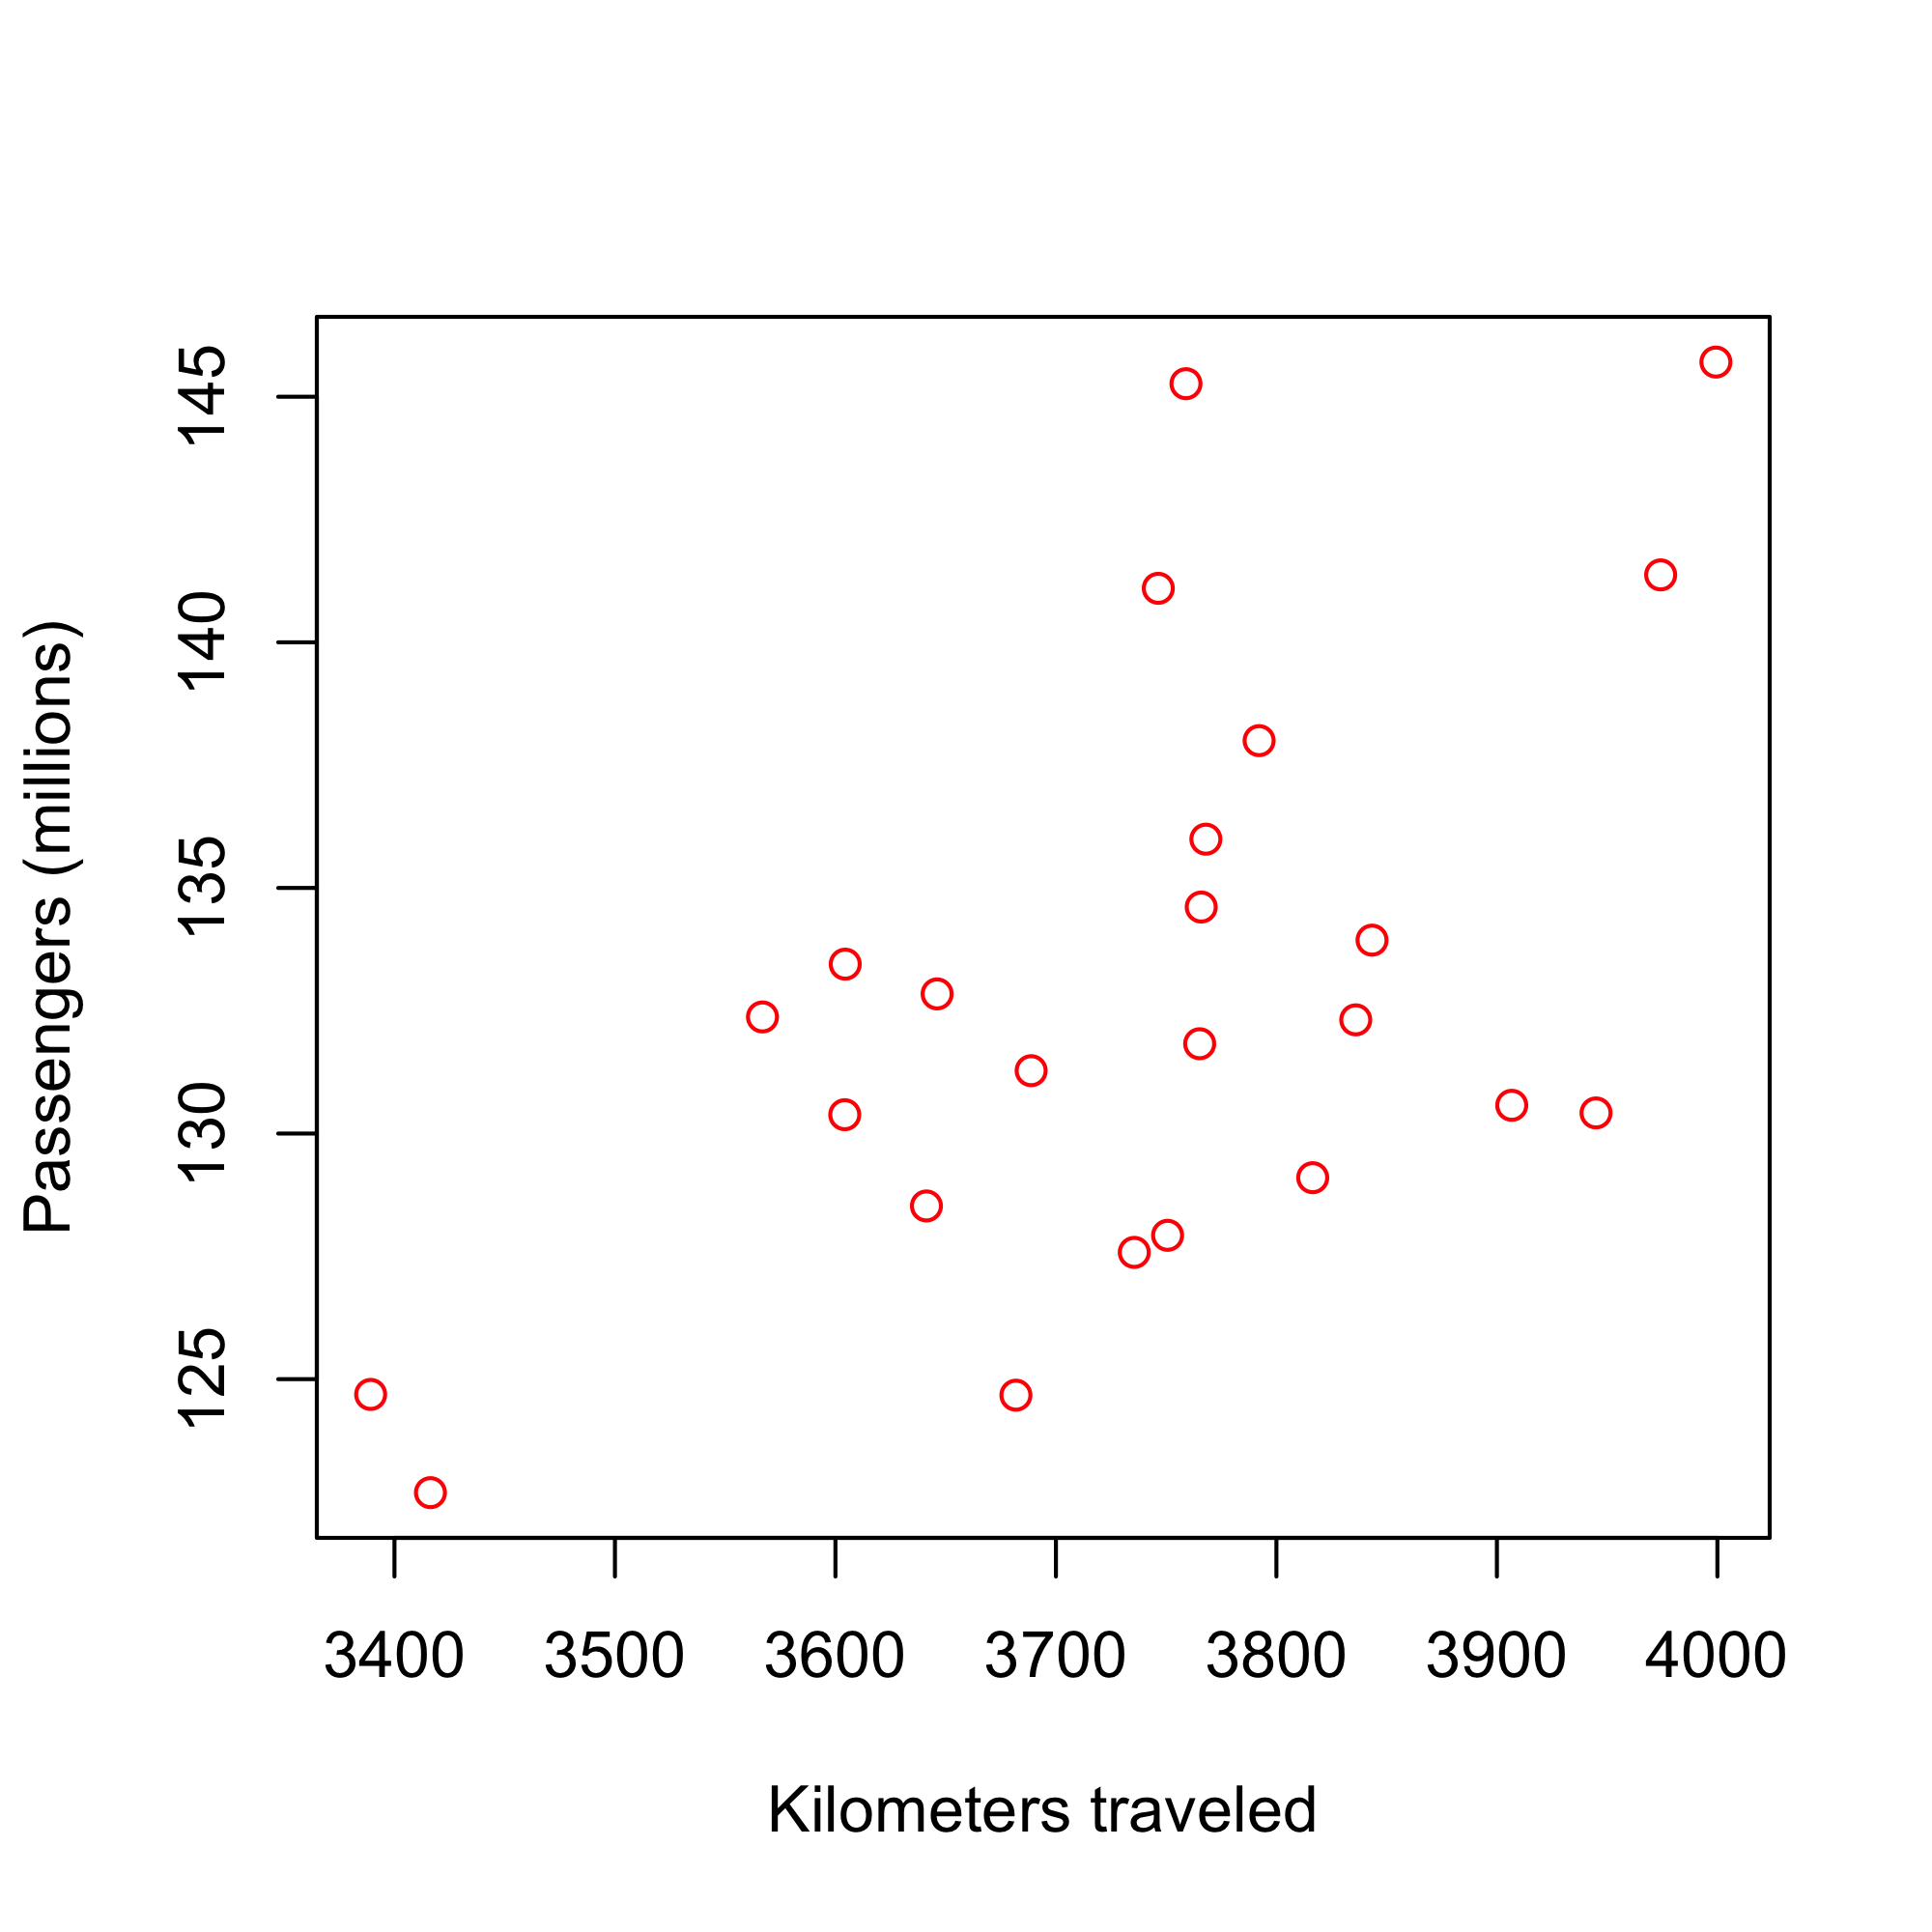
\includegraphics[width=0.3\linewidth]{correlation_km_passng}
 	\caption{Plot of kilometers traveled against passengers transported.}
 	\label{fig:correlation}
 \end{figure}
 
 
 Among the non-parametric tests one can find $\chi^2$  tests, Spearman-Kendall correlation coefficients, and Kruskal-Wallis tests. A $\chi^2$ test is performed in Listing \ref{lst:chi} to see if two categorical variables are dependent, by means of a contingency table. The categorical variables are low and high kilometers traveled and energy consumption, defined as being below or above the median. The null hypothesis is that the variables are independent, which cannot be rejected with the obtained $p$-value (0.219). This is a weak indication of the variables being dependent.
  \begin{lstlisting}[language=R, caption={Chi Squared test.}, label={lst:chi} ]
df2 <- data.frame(km, kwh)

df2$cat_x <- (df2$km < median(km))

df2$cat_y <- (df2$kwh < median(kwh))

chisq.test(table(df2$cat_x, df2$cat_y), correct = FALSE) 

#Pearson's Chi-squared test

#data:  table(df2$cat_x, df2$cat_y)
#X-squared = 1.5105, df = 1, p-value = 0.2191
 \end{lstlisting}
 
 Other examples of statistical tests are shown next. In Listings \ref{lst:two-sample-t} and \ref{lst:wilcoxon-rank-sum}, a null hypothesis of whether the number of passengers transported in 2018 has the same mean as the number of passengers transported in 2019 is tested. The difference between these two tests is that the $t$-test assumes the samples are drawn from a normal distribution, while Wilcoxon rank-sum test does not. In both tests, a $p$-value larger than 0.05 is obtained, so the null hypothesis cannot be rejected, suggesting both samples may have the same mean.
  
  \begin{lstlisting}[language=R, caption={Two sample t-test.}, label={lst:two-sample-t} ]
t.test(passng18, y=passng19)

#Welch Two Sample t-test

#data:  passng18 and passng19
#t = -0.087937, df = 21.716, p-value = 0.9307
#alternative hypothesis: true difference in means is not equal to 0
#95 percent confidence interval:
#-5.468207  5.023664
#sample estimates:
#mean of x mean of y 
#132.6653  132.8876 
 \end{lstlisting}
 
 \begin{lstlisting}[language=R, caption={Wilcoxon rank sum test.}, label={lst:wilcoxon-rank-sum} ]
 wilcox.test(passng18, passng19, alternative = "g")
 
 #Wilcoxon rank sum exact test
 
# data:  passng18 and passng19
#W = 68, p-value = 0.6006
#alternative hypothesis: true location shift is greater than 0
 \end{lstlisting}
 
 In Listing \ref{lst:kolmogorov-smirnov}, a null hypothesis of whether the number of passengers transported in 2018 and in 2019 come from the same distribution is tested. A $p$-value of 0.99 is obtained, which suggests the data indeed comes from the same distribution. 
 \begin{lstlisting}[language=R, caption={Kolmogorov Smirnov test.}, label={lst:kolmogorov-smirnov} ]
 ks.test(passng18, passng19)
 
#Two-sample Kolmogorov-Smirnov test
 
#data:  passng18 and passng19
# D = 0.16667, p-value = 0.9985
# alternative hypothesis: two-sided
 \end{lstlisting}
 


\subsubsection{Further considerations}
The \textbf{choosing of significance level} $\alpha$ should depend on how dangerous is to reject $H_0$ when it is true, with lower $\alpha$ values associated with a lower risk tolerance \cite{spiegel}. Navarro mentions in her book \cite{Navarro} that a \textbf{common mistake} is thinking the $p$-value is the probability of the null hypothesis to be true. \textbf{Statistical power} refers to the probability of rejecting the null hypothesis when it is false \cite{Everitt_2002}. It gives a method of discerning between competing tests of the same hypothesis, with the test with the higher power being preferred \cite{Everitt_2002}. 

\section{Conclusion}
Statistical hypothesis tests give an important set of tools to use when working with data, as is usually done in many scientific domains. Assumptions and conclusions must be carefully looked at, to avoid reaching to erroneous conclusions. 

\appendix
\section{Guide} \label{appendix}
Part of a guide for choosing the correct statistical test, created by the UCLA's Institute for Digital Research and Education \cite{idre_stats}, is shown in Table \ref{tab:guide}.

\begin{table}
	\centering
	\caption{Guide for choosing statistical tests.}
	\begin{tabular}{p{0.1\textwidth} | p{0.2\textwidth} | p{0.3\textwidth} | p{0.3\textwidth}}
		\hline
		Number of dependent variables & Nature of Independent Variables (IVs) & Nature of Dependent Variable(s) & Test(s) \\
		\hline
		1 & Zero IVs (1 population) & interval and normal & one-sample t-test \\
		 & & ordinal or interval & one-sample median \\
		 & & categorical (two categories) & binomial test \\
		 & & categorical & Chi-square goodness-of-fit \\
		\hline
		1 & One IV with two levels (independent groups) & interval and normal & two independent sample t-test \\
		 & & ordinal or interval & Wilcoxon-Mann Whitney test\\
		 & & categorical & Chi-Square test, Fisher's exact test \\
		\hline
		1 & One IV with two or more levels (independent groups) & interval and normal & one-way ANOVA\\
		 & &ordinal or interval & Kruskal-Wallis \\
		 & & categorical & Chi-square test\\
		\hline
		1 & One IV with two levels (dependent / matched groups) & interval and normal & paired t-test \\
		 & & ordinal or interval & Wilcoxon signed ranks test \\
		 & & categorical & McNemar \\
		 \hline
		 1 & Two or more IVs (independent groups)  & interval and normal & factorial ANOVA\\
		  & & ordinal or interval & ordered logistic regression \\
		  & & categorical (two categories) & factorial logistic regression\\
		 \hline 
		 1 & One interval IV & interval and normal & correlation, simple linear regression \\
		 & & ordinal or interval & non-parametric correlation \\
		 & & categorical & simple logistic regression\\
		 \hline
	\end{tabular}
\label{tab:guide}
\end{table}

%%%%%%%%%%%%%%%%%%%%%%%%%%%%

\bibliographystyle{siam}
\bibliography{refr}


%%%%%%%%%%%%%%%%%%%%%%%%%%%%
\end{document}
